\documentclass{beamer}
\usepackage[utf8]{inputenc}
\usepackage[russian]{babel}
\usepackage{amsmath,mathrsfs,mathtext}
\usepackage{graphicx, epsfig}
\usepackage{placeins}
\DeclareMathAlphabet\mathbfcal{OMS}{cmsy}{b}{n}
\usetheme{Warsaw}%{Singapore}%{Warsaw}%{Warsaw}%{Darmstadt}
\usecolortheme{sidebartab}
\setlength\headheight{10pt}
\definecolor{beamer@blendedblue}{RGB}{15,120,80}
%----------------------------------------------------------------------------------------------------------
\title[\hbox to 56mm{Тематический поиск схожих дел\hfill\insertframenumber\,/\,\inserttotalframenumber}]
{Тематический поиск схожих дел в коллекции актов арбитражных судов}
\author[Н.\,А. Герасименко]{\large \\Герасименко Николай Александрович}
\institute{\large
Московский авиационный институт}

\date{\footnotesize{\emph{Курс:} Численные методы обучения по прецедентам\par (практика, В.\,В. Стрижов)/Группа 8О-103М, весна 2019}}
%----------------------------------------------------------------------------------------------------------
\begin{document}
%----------------------------------------------------------------------------------------------------------
\begin{frame}
%\thispagestyle{empty}
\titlepage
\end{frame}
%-----------------------------------------------------------------------------------------------------
\begin{frame}{Цель исследования}
\begin{block}{Цель работы}
	Решение задачи информационного поиска по коллекции актов арбитражных судов.
    \end{block}
\begin{block}{Проблема}
	Специалисты в области юриспруденции вынуждены тратить большое количество времени на поиск релевантной судебной практики.
    \end{block}
\begin{block}{Метод решения}
	Построение тематической модели коллекции с помощью открытой библиотеки BigARTM, реализующей вероятностное тематическое моделирование на основе аддитивной регуляризации.
    \end{block}
\end{frame}
%----------------------------------------------------------------------------------------------------------
\begin{frame}{Литература}
Теория АРТМ:
    \begin{itemize}
        \item Konstantin Vorontsov and Anna Potapenko. Additive regularization of topic models. Machine Learning, 2015.
    \end{itemize} 
Библиотека BigARTM:
    \begin{itemize}
        \item Konstantin Vorontsov, Oleksandr Frei, Murat Apishev, Peter Romov, and Marina Dudarenko. Bigartm: open source library for regularized multimodal topic modeling of large collections.
In International Conference on Analysis of Images, Social Networks and Texts, pages 370-381. Springer, 2015.
    \end{itemize} 
Опорное исследование:
    \begin{itemize}
        \item Anastasia Ianina, Lev Golitsyn, and Konstantin Vorontsov. Multi-objective topic modeling for exploratory search in tech news. In Communications in Computer and Information Science, pages 181-193. Springer International Publishing, nov 2017.
    \end{itemize} 
\end{frame}
%----------------------------------------------------------------------------------------------------------
\begin{frame}{Постановка задачи}
\begin{block}{Дано}
%$(d_{i},w_{i},t_{i})_{i=1}^{n} \sim p(d,w,t)$, где
	Коллекция текстовых документов $D$
    \begin{itemize}
        \item $n_{dw}$~--- частоты терминов $w$ в документах коллекции $d \in D$.
Термины относятся к одному из трех типов, называемых модальностями: слово естественного языка, ссылка на НПА, юридический термин.
    \end{itemize} 
    \end{block}
\begin{block}{Найти}
	Параметры тематической модели $p(w|d)=\sum\limits_{t \in T} {\phi_{wt}\theta_{td}}$
    \begin{itemize}
        \item $\phi_{wt}$~--- вероятности терминов $w$ в темах $t \in T$.
        \item $\theta_{td}$~--- вероятности тем $t$ в каждом документе $d \in D$.
    \end{itemize} 
Поставлена задача стохастического матричного разложения.
	%Максимизируя логарифм правдоподобия с регуляризатором:
%\begin{align*}
%	\sum\limits_{d,w} {n_{dw}ln\sum\limits_{t \in T}} {\phi_{wt}\theta_{td}}+R(\Phi,\Theta)\to \max
%\end{align*} 
    \end{block}
%\begin{block}{Внешний критерий качества}
%	Специалисты в области юриспруденции вынуждены тратить большое количество времени на поиск релевантной судебной практики.
   % \end{block}
\end{frame}
%----------------------------------------------------------------------------------------------------------
\begin{frame}{Необходимость регуляризаторов}
\begin{block}{Оптимизационная задача в АРТМ}
	Для каждой модальности вводится критерий логарифма правдоподобия и с помощью EM-алгоритма максимизируется их взвешенная сумма.
\begin{align*}
	\sum\limits_{d,w} {n_{dw}\ln \sum\limits_{t \in T}} {\phi_{wt}\theta_{td}}+\sum\limits_{i}\tau_{i}R_{i}(\Phi,\Theta)\to \max
\end{align*} 
    \end{block}
\begin{block}{Регуляризаторы $R_{i}$}
	Добавляются к сумме как дополнительные критерии c \\*весами $\tau_{i}$, являющимися гиперпараметрами модели. Регуляризаторы необходимы, поскольку в общем случае задача имеет бесконечно много решений.
    \end{block}
\end{frame}
%----------------------------------------------------------------------------------------------------------
\begin{frame}{Используемые регуляризаторы}
\begin{block}{Регуляризаторы сглаживания и разреживания}
	Данные два регуляризатора имеют одинаковый вид и отличаются только знаками коэффициентов $\alpha$ и $\beta$, для регуляризатора разреживания они отрицательны.
\begin{align*}
R(\Phi,\Theta)=\beta \sum_{m \in M}\sum_{t \in T}\sum_{w \in W^m} \beta_{w} \ln \phi_{wt} + \alpha \sum_{d \in D}\sum_{t \in T}\alpha_{t} \ln\theta_{td}\to \max.
\end{align*} 
    \end{block}
\begin{block}{Регуляризатор декоррелирования}
Вводит в модель требование различности тем путем минимизации ковариации между столбцами матрицы $\Phi$.
\begin{align*}
R(\Phi)=-\tau \sum_{t \in T}\sum_{s \in T\backslash t}\sum_{w \in W} \phi_{wt}\phi_{ws} \to \max.
\end{align*} 
    \end{block}
\end{frame}
%----------------------------------------------------------------------------------------------------------
\begin{frame}{Внешний критерий качества}
%\begin{block}{Используемая информация}
%	Для оценки качества построения векторных представлений документов коллекции используем информацию о принадлежности каждого документа определенной категории дел таких как, например, <<Особенности банкротства отдельных категорий должников>> или <<Внешнее управление>>.
 %   \end{block}
\begin{block}{Идея}
	Рассчитаем согласованность картины кластеризации векторных предствлений документов с известной нам картиной классификации документов по категориям. В качестве критериев согласованности используем критерии ARI и AMI.
    \end{block}
\begin{block}{Adjusted Rand Index (ARI)}
%\begin{align*}
\begin{center}
	$ARI(U,V)={RI-E\{RI\}\over{\max{\{RI\}}-E\{RI\}}}$
\end{center}
%\end{align*} 
    \end{block}
\begin{block}{Adjusted Mutual Information (AMI)}
\begin{center}
	$AMI(U,V)={MI(U,V)-E\{MI(U,V)\}\over{\max{\{H(U),H(V)\}}-E\{MI(U,V)\}}}$
\end{center} 
    \end{block}
\end{frame}
%----------------------------------------------------------------------------------------------------------
\begin{frame}{Внутренние критерии качества}
%\begin{block}{Используемая информация}
%	Для оценки качества построения векторных представлений документов коллекции используем информацию о принадлежности каждого документа определенной категории дел таких как, например, <<Особенности банкротства отдельных категорий должников>> или <<Внешнее управление>>.
 %   \end{block}
\begin{block}{Перплексия языковой модели}
	Мера неопределенности терминов в тексте.
\begin{align*}
	%\mathcal{P}(D) =
 \exp(-{1\over{n}}\sum\limits_{d,w} {n_{dw}}\ln p(w|d)),~n=\sum\limits_{d,w}{n_{dw}}
\end{align*} 
    \end{block}
\begin{block}{Разреженность распределений терминов в темах}
	Отвечает гипотезе разреженности.
	
Равен количеству элементов матрицы $\Phi$, меньших заранее заданного порога $\epsilon=$ const.
    \end{block}
\end{frame}
%----------------------------------------------------------------------------------------------------------
\begin{frame}{Стратегия регуляризации}
%\begin{block}{Общий подход к подбору гиперпараметров}
%Выбор гиперпараметров модели производился из заданной сетки значений по нескольким критериям качества: перплексии, разреженности распределений токенов в темах, а также солгласованности с известной картиной классификации.
 %   \end{block}
\begin{block}{Порядок добавления регуляризаторов и выбор гиперпараметров}
    \begin{itemize}
        \item[1] Производим 8 итераций EM-алгоритма с регуляризатором декоррелирования для каждого значения коэффициента регуляризации декоррелирования из сетки значений. Выбираем лучший коэффициент регуляризации для регуляризатора декоррелирования.
        \item[2] Добавляем регуляризатор разреживания распределений тем в документах. Производим еще 8 итераций EM-алгоритма с обоими регуляризаторами и выбираем лучшее значение коэффициента регуляризации.
    \end{itemize} 
    \end{block}
\begin{block}{Критерии качества}
\begin{itemize}
 \itemПерплексия, 
\itemРазреженность распределений терминов в темах.
\itemСолгласованность с известной картиной классификации.
    \end{itemize} 
\end{block}
\end{frame}
%----------------------------------------------------------------------------------------------------------
\begin{frame}{Вычислительный эксперимент  \\*Внутренние критерии качества}
\begin{figure}
	Зависимость перплексии и разреженности матрицы $\Phi$ от количества итераций
      \vspace{0.01em}\begin{tabular}{p{4.4cm} p{4.5cm}}
        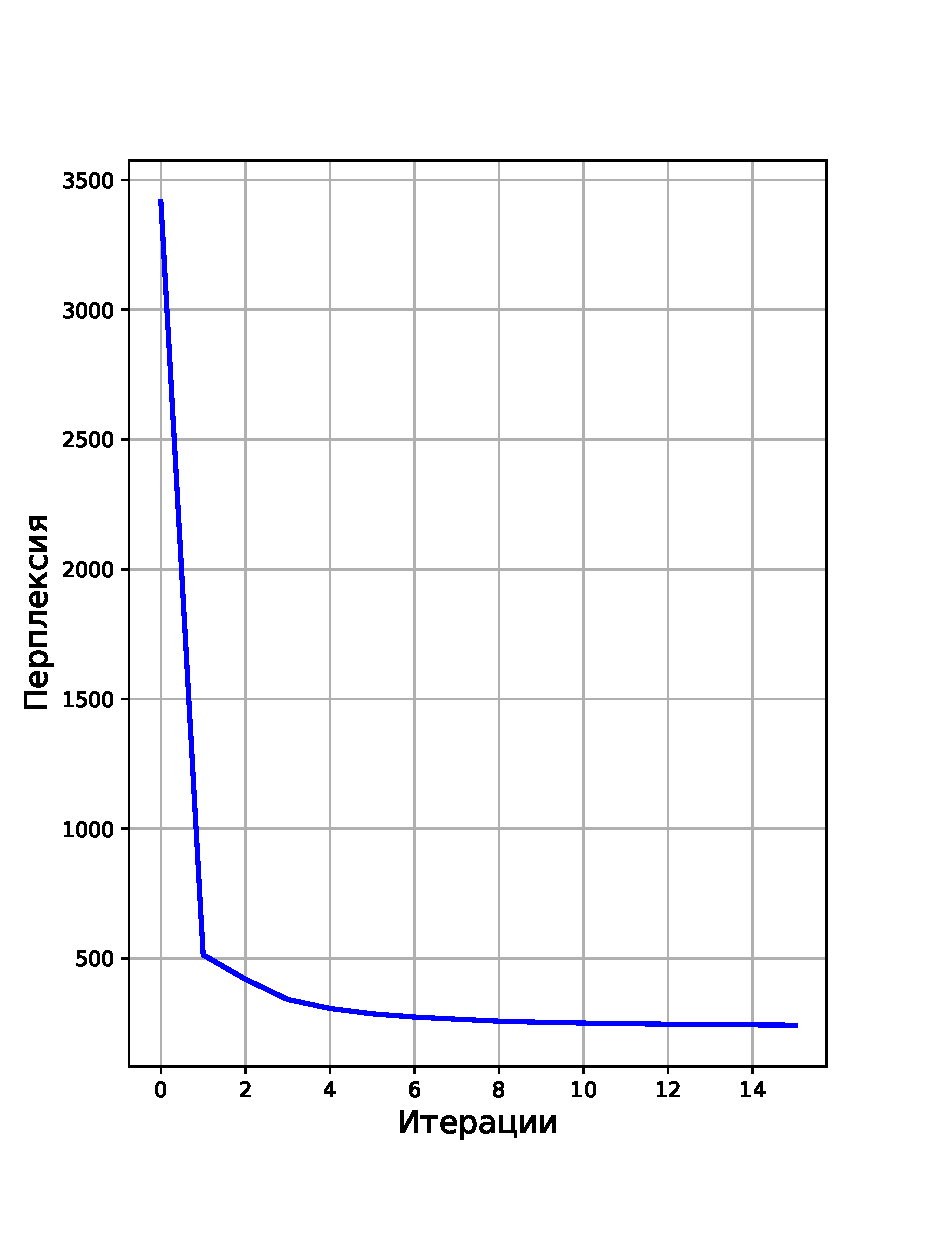
\includegraphics[width=4.7cm]{perplexity}
         &
        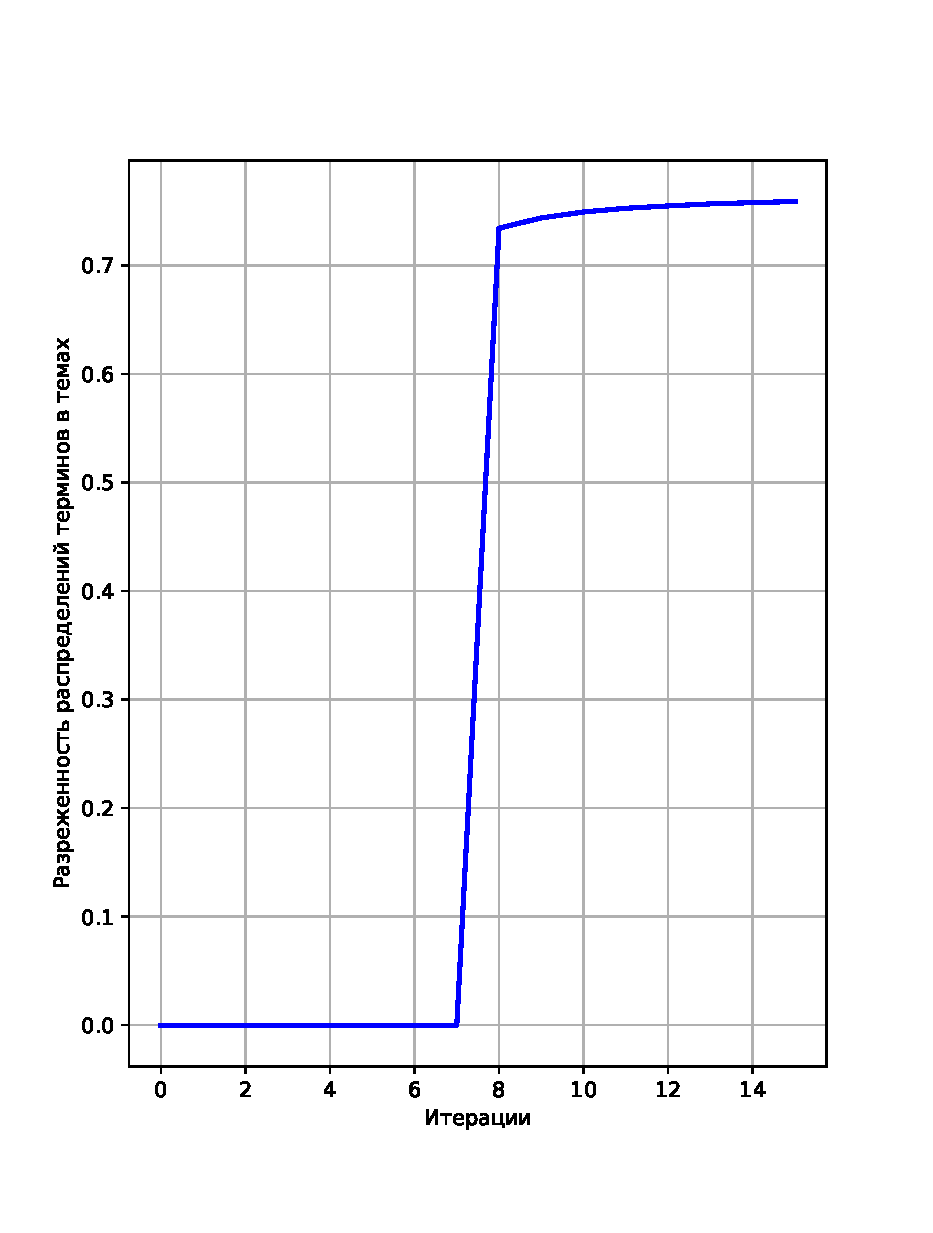
\includegraphics[width=4.7cm]{sparseTheta}
         \end{tabular}
\end{figure}
\end{frame}
%----------------------------------------------------------------------------------------------------------
\begin{frame}{Вычислительный эксперимент \\*Внешние критерии качества}
\begin{block}{Сравнение с базовыми алгоритмами}
	Для оценки качества модели были использованы в качестве базовых алгоритмов  
    \begin{itemize}
        \item TF-IDF по словам 
        \item TF-IDF по выделенным из текста ссылкам на нормативно-правовые акты (НПА), например, \\*<<пункт 3 статьи 6 УК РФ>>.
    \end{itemize} 
    \end{block}

\begin{table}[H]
% \caption{\label{tab:summary}Сравнение показателей внешнего критерия качества.}
\begin{center}
\begin{tabular}{|c|c|c|}
\hline
Модель & ARI & AMI\\
\hline
TF-IDF по словам & 10\% & 12.5\% \\
\hline
TF-IDF по ссылкам на НПА & 17\% & 22\% \\
\hline
BigARTM & 37.5\% & 42\% \\
\hline
\end{tabular}
\end{center}
\end{table}
\end{frame}
%----------------------------------------------------------------------------------------------------------
\begin{frame}{Заключение}
\begin{itemize}
\item При помощи библиотеки BigARTM построена тематическая модель, строющая для документов коллекции сжатые векторные представления и, таким образом, позволяющая реализовать поиск, используя косинусную меру близости.

\item Был реализован метод внешней оценки качества тематической модели, заключающийся в вычислении согласованности между картиной кластеризации тематических векторов документов коллекции и их принадлежности различным категориям дел.

\item Результаты показывают, что тематическая модель способна корректно строить векторные представления юридических документов, что, в перспективе, дает возможность построения системы разведочного поиска, с использованием тематического моделирования в качестве ключевой технологии.
    \end{itemize} 
\end{frame}
%----------------------------------------------------------------------------------------------------------
\end{document} 